\documentclass{article}
\usepackage{iclr2021,times}
\iclrfinalcopy % Camera ready version!

\usepackage[utf8]{inputenc}
\usepackage[T1]{fontenc}

\usepackage[hyphens]{url}
\usepackage{hyperref}
\usepackage{graphicx}
\hypersetup{
    colorlinks,
    citecolor=blue,
    filecolor=blue,
    linkcolor=blue,
    urlcolor=blue,
}
\usepackage{algorithm}
\usepackage{algorithmic} 

\usepackage{natbib}
\setcitestyle{authoryear,open={(},close={)}}

\usepackage{amsmath,amssymb}
\usepackage{makecell}
\usepackage{chngcntr} % make figure numbering in appendix work

\usepackage{caption}
% Small captions
\captionsetup[figure]{font=small,labelfont=small}

%%% SPACE-REDUCING HACK 1/2
% Reduce spacing around floats 
\setlength{\floatsep}{8pt plus 4pt minus 4pt}
\setlength{\textfloatsep}{8pt plus 4pt minus 3pt}

\usepackage{xcolor}
\bibliographystyle{iclr2021}


\title{Planetary Nebulae Classification from Limited Labeled Dataset \\ Checkpoint 2}
\author{Joseph Hadidjojo \And Tung Pham \And Arman Muratbayev}

\begin{document}

\maketitle

\textbf{Instructions for Checkpoint 2:} ~~\url{https://www.cs.tufts.edu/cs/152L3D/2024f/project_checkpoint2.html}


\section*{A: Changelog}

Since the last milestone (project pitch), we have changed:
\begin{itemize}
    \item Data: Cropped dataset down to 224 x 224 from 256 x 256 to ease training time
    \item Method: Decided to implement MixMatch for Pseudo-labeling (after OH discussion)
\end{itemize}

\section*{B: Challenges}
At the moment, our biggest roadblocks are:
\begin{enumerate}
    \item Preliminary Implementation of MixMatch
    \item Completing Hyperparameter Search for Baseline and LP-FT model
\end{enumerate}

We'd like instructor help with the following: (for urgent questions, please also make a Piazza post)
\begin{itemize}
    \item Sanity-check: Validating MixMatch understanding and implementation
\end{itemize}

\section*{C: Timeline}

How will you have preliminary experiments all completed by the slides due date on 12/10?

\begin{table}[!h]
    \begin{tabular}{p{10cm} p{1cm} p{2cm}}
    \textbf{Task} & 
    \textbf{Target Date} & 
    \textbf{Assigned to}
    \\
    Finalize MixMatch Implementation& 11/26 & Arman, Tung
    \\
    Finalize Hyperparameter search for Baseline and LP-FT models & 11/27 & Joseph
    \\
    Begin Hyperparamater search for MixMatch & 11/27 & Arman, Tung, Joseph
    \\
    Begin data compilation, report and slides preparation & 12/3 & Joseph
    \end{tabular}
\end{table}

\newpage

\section{Introduction}

{\color{red} Adapt from Checkpoint 1}

\subsection{Prediction Task}
% TODO Paragraph 1: What's the prediction task?

Planetary nebulae (PNe) represent a late stage in the life cycle of medium-mass stars, marked by glowing elliptical objects of ionized gas. Accurately distinguishing true PNe from visually similar non-PNe objects is challenging due to the overlap in visual characteristics (such as shape and luminosity) with other types of nebulae and celestial bodies. Given this context, this project aims to classify True vs Rejected PNes from 3-channel (RGB), 224 x 224 deep-space images of glowing, elliptical space objects.

\subsection{Overall Goal}
% TODO Paragraph 2: What's your overall goal?

This project aims to build upon prior work (\cite{awangiskandar2020}) that first applied a Transfer Learning (Linear Probing) approach toward PNe classification (achieving over 80\% prediction accuracy). Our objectives are twofold: first, to reproduce the original results as a benchmark, and second, to explore whether more advanced methods—such as Linear Probing with Fine-Tuning (LP-FT) and MixMatch Pseudo-Labeling—can push this accuracy even higher. This work is exciting as it not only attempts to validate pioneering Transfer Learning techniques within the Astrophysical context, but also tests innovative adaptations that may set new standards in identifying PNes with greater precision. Positive results from this project may motivate Astronomers to more readily explore and adopt ML techniques during deep-space explorations and analysis.

\subsection{Methods}
% TODO Paragraph 3: Introduce the methods you'll study.

This project leverages Transfer Learning, where models pre-trained on large datasets (ImageNet) are adapted to specialized tasks, enhancing performance with minimal labeled data (\cite{pan2010survey}). The primary methods include Linear Probing (LP), which retrains only the final layer of the model, and  Linear Probing with Fine-Tuning (LP-FT),  which hopes to further improve accuracy by fine-tuning deeper layers (\cite{kumar2022lpft}). Additionally, we implement MixMatch pseudo-labeling (\cite{lee2013pseudo}) to generate ``soft'' labels for unlabeled data, allowing the model to train on a larger, unlabeled dataset. Due to the nature of our dataset, we will be performing properties augmentation (colorspace, brightness, contrast) instead of physical augmentation (rotational, translational, cropping).

While LP is computationally efficient, its adaptability is limited, potentially capping model performance. LP-FT, in contrast, offers greater flexibility and accuracy by adjusting multiple layers, though it increases training complexity and the risk of overfitting if not carefully tuned. Pseudo-labeling boosts accuracy further by including additional data, but it can introduce label noise, especially when initial predictions are uncertain. This project will balance these trade-offs---accuracy, computational costs, and training stability---to identify the most effective approach for PNe classification.

\subsection{Hypothesis}
% TODO Paragraph 4: Specific hypothesis

The hypothesis for this experiment is that a \textbf{combination of Linear Probing and Fine-Tuning (LP-FT) on a pre-trained model will outperform independent MixMatch Pseudo-labeling in classification accuracy of True or Rejected PNe}. 

Our hypothesis is largely based on MixMatch's reliance of consistency regularization towards different input perturbations. Given the nature of our dataset (low-resolution images of deep-space elliptical objects, often procured by cropping certain regions of interest from original deep-space image), we hypothesize that the MixMatch method might not be able to extract enough discriminative representations of True PNes from image transformations/augmentations alone to pseudo-label the unlabeled dataset effectively. However, should MixMatch prove to be able to pseudo-label effectively, we acknowledge that it might be able to outperform the LP-FT model due to the fact that it will be able to leverage the unlabeled portion of our dataset which LP-FT would not.

% Neither LP-FT nor MixMatch pseudo-labeling alone is likely to achieve optimal results. While LP-FT alone provides a robust baseline by leveraging features learned from large datasets, it still relies solely on the limited labeled dataset, restricting the model's exposure to potential variations and unique features in True vs. Rejected PNe. MixMatch Pseudo-labeling, on the other hand, heavily depends on the initial model’s performance to generate accurate pseudo-labels. Without the specialized feature adaptation from LP-FT, pseudo-labeling may reinforce misclassifications. Thus, combining LP-FT with pseudo-labeling fills in the limitations of each approach: LP-FT provides the nuanced feature adaptation, while pseudo-labeling extends the dataset, enhancing the model’s generalization capabilities across PNe variations.

Other approaches commonly used for learning with limited labeled data, such as Contrastive Self-Supervised methods, may be less appropriate in this context. As an example, SimCLR, which rely on data augmentations and contrastive pairs, may struggle with low-resolution PNe images and noise from nearby bright stars, leading to potentially learning artifacts rather than meaningful features. By contrast, LP-FT with pseudo-labeling allows for more precise, label-driven adaptation, effectively addressing both the complex nature of the dataset and the limited availability of labeled samples, making it the most suitable strategy for this classification task.

\section{Methods}

{\color{red} Leave blank for Checkpoint 2. Focus on Sec 3 and 4 below.}

\section{Data and Experimental Plan}

{\color{red} Adapt from Checkpoint 1}

\subsection{Data description}
To create our dataset, we will scrape Optical Images of possible PNes from the SuperCOSMOS Sky Survey (SSS), as compiled and hosted by the \textbf{\textit{H}}ong Kong/Australian \textbf{\textit{A}}stronomical Observatory/ \textbf{\textit{S}}trasbourg Observatory \textbf{\textit{H}}-alpha Planetary Nebula (HASH-PN) research platform database (which we will from here on refer to as HashDB). HashDB compiles over 30,000 deep-space images of possible or suspected PNes, of which only a fraction of them are labeled as "True PNe" (independently confirmed to be a Planetary Nebulae). The remaining images are either unlabeled (indicating "Possible PNe") or labeled as "Rejected PNe" (independently confirmed to be other types of Nebulae) (\cite{parker2016hash}). These images are also of different modalities, and are grouped based on the equipment and method used to capture the respective images (e.g., Optical, Quotient, WISE342).


Our dataset consists of 1,000 sub-samples from the HashDB 'Optical' group subset, which are 3-channel RGB images in nature. The exact sampling and resulting dataset properties will be discussed further in the section 3.3 below. \colorbox{orange}{Need to fix GradeScope notes \& update to Cp2 specifications. Possibly Done?}

\subsection{Performance metric}
For this experiment, the primary performance metric will be \textbf{classification accuracy}, which measures the proportion of PNe images correctly classified as True or Rejected. This metric is appropriate as the primary goal of the experiment is to maximize correct identifications of PNe types.

We will also track \textbf{AUROC} to measure the model’s ability to distinguish True PNe from Rejected PNe across different thresholds to provide a clear view of the model's discriminative performance.

Furthermore, While we have attempted to keep our dataset balanced with a 50/50 distribution of True and Rejected PNe, we will also track the \textbf{F1-score} for each class. The F1-score balances precision and recall, which will help us identify if the model favors one class over the other.

\subsection{Splitting Data to train/tune/assess generalization.}
{\color{red} This one a new paragraph, probably need more than just copy pasting}

As mentioned previously, our dataset was built using 1,000 sub-samples of the HashDB 'Optical' group subset. The first 500 of this dataset are evenly sampled from both the "True PNe" and "Rejected PNe" labeled images to create an evenly distributed labeled dataset for use in our Baseline and LP-FT method. The remaining 500 are sampled from HashDB's unlabeled pool to create an unlabeled dataset for our Pseudo-labeling method. While we acknowledge that this might not be the best representation of 'True' vs. 'Rejected' PNes in space, we also note the immense scale of the galaxy and the lack of knowledge in the distribution of PNes vs other Nebulaes. With this in mind, we constructed our dataset with the intention of mitigating possible complications and uncertainties that we currently have little knowledge of.

Both labeled and unlabeled datasets will be split into a Train/Test/Validate set for the purpose of training, hyperparameter tuning, and assessing generalization respectively. The split will be done in an 8:1:1 ratio, following the splits originally defined by \cite{awangiskandar2020}, but with an added emphasis on preventing data leakage which was not originally discussed in that paper.

To prevent data leakages, we will leverage the included DRAJ2000 and DDEC2000 values in the dataset, which represent the object's coordinates in space. These coordinates will be used to ensure that no two images with the same coordinates exist in the different data split. 

To further prevent leakage/overlap between phases, the labeled portion of the dataset is exposed only for the supervised training phase while the unlabeled portion is withheld only for the pseudo-labeling phase, ensuring that the pseudo-labeling phase does not inadvertently benefit from exposure to the same images.

% To further prevent leakage/overlap between phases, we will divide our 1,000 images into two groups: one dedicated to the LP-FT phase and another reserved for evaluating the pseudo-labeling phase. For the LP-FT phase, we plan to allocate approximately 50-60\% of the images for supervised training, while the remaining 40-50\% will be withheld for pseudo-label evaluation, ensuring that the pseudo-labeling phase doesn’t inadvertently benefit from exposure to the same images.

\begin{table}[!h]
    \centering
    \begin{tabular}{c|c}
         &  \\
         & 
    \end{tabular}
    \caption{Summary info about splits into train/val/test.}
    \label{tab:my_label}
\end{table}

\subsection{Training and hyperparameter tuning plan}

For each training phase of all three methods, we perform mini-batch gradient descent with PyTorch's Adam optimizer implementation \cite{paszke2019pytorch} with a fixed learning rate. Each training phase proceeds for up to 100 epochs. After every epoch, we record the cross-entropy loss on the validation set. If this value plateaus for 15 consecutive epochs, we stop the training phase early.

Both supervised and semi-supervised learning can be quite sensitive to hyperparameters. Our hyperparameter tuning plan includes tuning both shared hyperparameters (learning rate, batch size) and unique hyperparameters. For baseline and LP-FT, we will also search through 3 different model architectures (DenseNet, ResNet, Inception-ResNet) as well as model complexity (L2 regularization).
% Hyperparameters: Model architecture (DenseNet, MobileNetV2, InceptionResNet), Model Parameter (Learning Rate, Batch Sizes), Model Complexity (L2 regularization)

For each method, we execute a serial grid search over the specified hyperparameters. Due to the increasing demand for HPC computing time, we have formulated our grid search which is mindful of the realistic computing resources available: personal, consumer-level hardware that is available for 4-8 hours over a few days. Training is done with each configuration permutation until either an early stopping criteria is satisfied or the maximum number of epoch is reached. We track the best configuration in terms of validation-set performance every epoch.
% Tuning Strategy: For each architecture, implement grid search of ~3 possible values each. LR in log10s, batch sizes (16,32,63), L2 log10s.


\section{Results}

\begin{figure}[!h]
    \begin{tabular}{c c c}    
    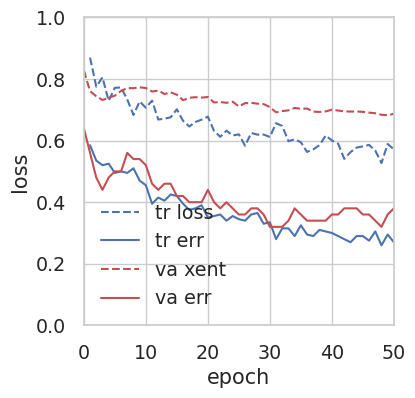
\includegraphics[width=0.25\textwidth]{Checkpoint2_Baseline.png}
    &
    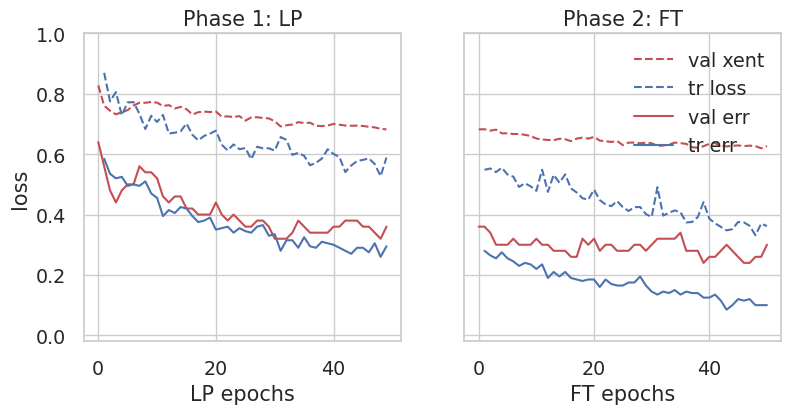
\includegraphics[width=0.48\textwidth]{Checkpoint2_LPFT.png}
    % &
    % \includegraphics[width=0.3\textwidth]{example-image-c.jpg}
    \end{tabular}
    \caption{\textbf{Proof of implementation progress.} Trace plots of Binary Cross-Entropy loss against Epochs for Baseline (LP) and LP-FT methods. These plots clearly illustrate how the FT-phase further lowers the loss over the LP-phase, indicating the validity of our implementation.}
\end{figure}



\begin{figure}[!h]
    \begin{tabular}{c r}
    Method & Classification Accuracy on Test set
    \\
    Baseline (Iskandar et. al.) & 86.0 (DenseNet-201)
    \\
    Baseline (Ours) & 71.2 (Preliminary)
    \\
    LP-FT (Ours) & 74.8 (Preliminary
    \\
    Mix-Match Pseudo-labeling (Ours) & 50
    % \\
    % LP-FT + Pseudo-labeling (Ours) & TBD
    \end{tabular}
    \caption{\textbf{Draft result.} Preliminary classification accuracy on Test set. These are preliminary results without hyperparameter tuning and using a simpler ResNet-10 architecture for the purpose of testing our implementation before investigating the more complex architectures we intended (Inception-ResNet, DenseNet). }
\end{figure}


\end{document}

